\chapter{Shingles}

  \subsection*{Premessa}
    Usare il classico algoritmo di ``string matching'' per determinare la similarità fra 2 documenti e' decisamente costoso computazionalmente. Esistono quindi altri metodi di rappresentare un documento che permettono di calcolare la similarità in modi diversi.

  \section{$k$-shingles}
    E' un metodo per la rappresentazione di un documento come un insieme di $k$-grammi, ovvero sottostringhe di lunghezza $k$.

    Costruiti i sottoset di $k$-grammi, si può calcolare la similarità tra due documenti tramite l'indice di Jaccard, ovvero la cardinalità dell'intersezione tra i due insiemi divisa per la cardinalità dell'unione.

    $$
      \text{Jaccard}(A, B) = \frac{|A \cap B|}{|A \cup B|}
    $$

    Tramite questa reinterpretazione, e' possibile avvalorale la similarità fra parole, in modo che pure parole che non sono perfettamente uguali (ad esempio ``player'' e ``players'') possano essere considerate simili.

    \subsection{Come scegliere $k$}
      La metrica $k$ deve essere scelta in base al documento che si vuole rappresentare. Minore e' $k$ e maggiore e' la probabilita' che un particolare $k$-gramma sia presente inoltre cresce la probabilita' che due documenti siano simili.

      E' importante ricordare che il numero di $k$-grammi dipende da $k$ e dalla lunghezza dell'alfabeto usato e cresce esponenzialmente.

      Ad esempio, usando un alfabeto generico di 27 caratteri (26 + spazio), il numero di $k$-grammi e' $27^k$.

  \section{Min-Hashing}
    Sebbene i $k$-grammi forniscano maggiore qualità rispetto al classico ``string matching'', si tratta di una metrica ancora troppo costosa.

    Un metodo abbastanza potente per ridurre notevolmente la dimensione della rappresentazione di un documento è l'uso di un algoritmo di hashing.

    Si consideri un documento $A$ come l'insieme dei suoi $k$-grammi. Il \textbf{min-hashing} di $A$ si definisce come l'elemento più piccolo di $A$ dopo l'applicazione di una permutazione casuale $\pi$. Pertanto il min-hashing di $A$ è dato da un elemento del set scelto casualmente da $\pi$. 

    Applicando la stessa permutazione ad ogni altro documento si ottengono i min-hashing di tutti i documenti.

    \begin{remark}
      I min-hash dei documenti $A$ e $B$ si denotano come $min(\pi_A)$ e $min(\pi_B)$.
    \end{remark}

    \begin{example}\label{ex:pi_perm}
      $$
      \begin{array}{ccc}
        \begin{array}{ccc}
          & A & B \\ \hline
          a & 1 & 0 \\
          b & 0 & 1 \\
          c & 0 & 0 \\
          d & 1 & 1 \\
          e & 0 & 1 \\
        \end{array}
        \ & \
        \begin{array}{ccc}
          \pi & A & B \\ \hline
          c & 0 & 0 \\
          d & 1 & 1 \\
          b & 0 & 1 \\
          e & 0 & 1 \\
          a & 1 & 0 \\
        \end{array}
      \end{array}
      $$

      La prima tabella rappresenta il documento $A$ e il documento $B$ come insiemi di $k$-grammi. La seconda tabella $A$ e $B$ dopo l'applicazione della permutazione $\pi$.
    \end{example}

    Per calcolare il min-hash dei due documenti è sufficiente scorrere la matrice dall'alto verso il basso seguendo l'ordine della permutazione $\pi$ e prendere la prima riga che contiene un $1$.

    Si nota poi con $x$ il numero di righe in cui entrambi i documenti presentano un $1$, mentre con $y$ il numero di righe in cui \textit{esattamente uno dei due documenti} presenta un $1$. Si scartano quindi le righe in cui entrambi i documenti presentano un $0$.

    Pertanto la probabilità che i due documenti siano simili e che pertanto il loro min-hash sia il medesimo è data dalla probabilità che la prima riga incontrata sia una con $1$ in entrambi i documenti.

    $$ p = \frac{x}{x + y} $$

    \begin{remark}
      Non è strettamente necessario eseguire l'intera permutazione, bensì è sufficiente generare una scelta casuale per la prima riga, scegliendola da quelle contate da $x$ o da $y$.
    \end{remark}

    \subsection{Min-hash Signatures}
      Purtroppo il metodo di min-hash non è così affidabile. Infatti sebbene possa dire che due documenti abbiano una certa probabilità di essere simili, non è in grado di dire quanto siano simili.

      Per superare questa limitazione, si possono usare più permutazioni, quindi calcolare più min-hashes. Supponendo di avere un set di permutazioni 
      $$\pi_1, \pi_2, \dots, \pi_n$$
      si può calcolare la similarità costruendo il vettore

      $$ \left[ \min(\pi_A^1), \min(\pi_A^2), \dots, \min(\pi_A^n) \right] $$

      per ogni documento. Ogni vettore che rappresenta un documento è detto \textbf{signature}. Questo tipo di ``firma'' può essere utilizzato per fornire una stima della similarità tra due documenti.

      Prendendo $k$ il numero di min-hash uguali, calcolate da $m$ permutazioni diverse per $A$ e $B$, allora l'indice di similarità è dato da
      $$ \text{Jaccard}(A, B) \approx \frac{k}{m} $$

      Ovviamente il tradeoff è che più permutazioni si usano e più la similarità è precisa, ma più è costoso il calcolo. In generale si vuole mantenere $m$ inferiore alla media di termini contenuti in un documento.

  \section{Hashing con sensibilità locale (LSH)}
    Pure tramite il min-hashing il costo computazionale può risultare troppo elevato. È necessario un metodo che permetta di eseguire una ricerca più rapida, mantenendo tuttavia un'alta probabilità che se due documenti sono simili, allora il loro min-hash sia lo stesso.

    Per farlo si può suddividere il set di min-hash $m$ in $b$ blocchi di $r=m/b$ elementi ciascuno. Ogni blocco è quindi un vettore di $r$ elementi. Ognuno di essi viene poi concatenato e nuovamente hashato, in modo da ottenere un nuovo vettore detto ``super-signature'' o ``super-shingle''

    In questo modo si salvano i documenti in hash-tables basate sulle super-signatures. Inoltre si utilizzano $b$ tabelle diverse, in modo da mantenere indipendentemente le $b$ super-signatures.

    Il funzionamento dell'algoritmo è il seguente:	
    \begin{enumerate}
      \item Si calcolano le min-hash di un documento $A$
      \item Si calcolano le $b$ super-signatures di $A$
      \item Si usano le super-signatures per accedere alle hash-tables
      \item Si recuperano i documenti associati a tali hash-tables
      \item Si ritorna l'unione di tutti i documenti recuperati
    \end{enumerate}

    Addizionalmente si può in seguito calcolare la similarità fra $A$ e i documenti con l'indice di Jaccard, il quale sebbene sia costoso, verrebbe applicato ad un sotto-set ristretto dei documenti, in modo da filtrare eventuali "falsi positivi".

    \clearpage

    \subsection{Similarity Hashing}
      Si consideri la seguente immagine, nella quale si vedono due documenti $A$ e $B$ come un vettore bidimensionale, dove i due vettori sono separati da un certo angolo $\theta$.

      \begin{figure}[h]
        \centering
        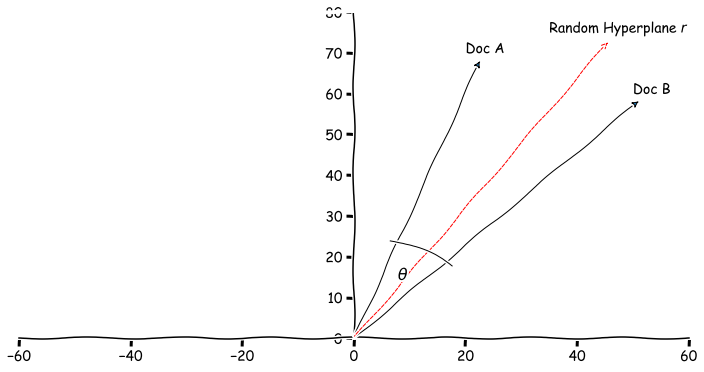
\includegraphics[width=1\textwidth]{images/sim-hash.png}
        \caption{Similarity Hashing}
      \end{figure}

      Preso un vettore casuale $r$ (un iperpiano se fossimo in uno spazio a più dimensioni), qual è la probabilità che $A$ e $B$ siano separati da $r$?

      Ponendo che l'angolo di $r$ può essere compreso fra $[0, 180]$ gradi, allora
      \begin{itemize}
        \item La probabilità che $r$ separi $A$ e $B$ è data da $\frac{\theta}{180}$
        \item Al contrario, la probabilità che $r$ non separi $A$ e $B$ è data da $\frac{180 - \theta}{180}$
      \end{itemize}

      \begin{remark}
        In pratica l'iperpiano $r$ rappresenta una firma composta da un singolo bit per un dato documento. Se il documento è al di sopra dall'iperpiano, allora il bit è $1$, altrimenti è $0$.
      \end{remark}

      Pertanto la probabilità che due documenti abbiano la stessa firma (quindi siano dallo stesso lato rispetto ad $r$) è data da
      $ \frac{\theta}{180} $

      \begin{remark}
        Dato un documento $A$ si può usare la seguente strategia
        \begin{enumerate}
          \item Si genera $r$ come una sequenza casuale di $+1$ e $-1$
          \item Si computa il prodotto scalare $r \cdot A$
          \item Se il risultato è positivo, allora si aggiunge un $1$ alla firma, altrimenti un $0$
          \item Si ripete il processo $m$ volte, ottenendo così una firma di $m$ bit
          \item Infine si può sfruttare la distanza di Hamming per calcolare la similarità fra due documenti
        \end{enumerate}
      \end{remark}

